\documentclass[conference]{IEEEtran}
\IEEEoverridecommandlockouts
\usepackage{cite}
\usepackage{amsmath,amssymb,amsfonts}
\usepackage{graphicx}
\usepackage{textcomp}
\usepackage{xcolor}
\usepackage{booktabs}
\usepackage{siunitx}
\usepackage{hyperref}

\title{Less Is More for 12-Lead ECG Classification: \\
       Anti-Aliased Decimation Raises a Plain 1D-CNN \\
       from \SI{88.43}{\percent} to \SI{97.34}{\percent} on Chapman--Shaoxing}

\author{\IEEEauthorblockN{Elaman Nazarkulov}
\IEEEauthorblockA{Department of Computer Engineering \\
Kyrgyz--Turkish Manas University \\
Bishkek, Kyrgyzstan \\
elaman.job@gmail.com}}

\begin{document}
\maketitle

\begin{abstract}
We revisit the common assumption that 12-lead electrocardiogram (ECG)
classifiers should consume the raw \SI{500}{\hertz}\,$\times$\,\SI{10}{\second}
input of \num{5000} samples per lead. Using the Chapman--Shaoxing corpus
(\num{45152} records, 78 multi-label classes) and an otherwise identical
baseline 1D convolutional neural network (1D-CNN), we measure the effect of
anti-aliased decimation of the input signal via \texttt{scipy.signal.decimate}.
Cutting the input length from \num{5000} to \num{500} samples (effective
\SI{50}{\hertz}) lifts test accuracy from \SI{88.43}{\percent} to
\SI{97.34}{\percent} (macro $F_1$ from \num{0.8713} to \num{0.9737}) while
reducing single-sample inference from \SI{89.88}{\milli\second} to
\SI{27.20}{\milli\second}. This one preprocessing change surpasses the
\SI{94.8}{\percent} accuracy target of the attention-hybrid configuration
that motivated the study --- without introducing attention, recurrent layers,
focal loss, or label re-balancing. The per-class failure set of the baseline
(11 labels with $F_1<0.60$, minimum \num{0.022}) recovers to $F_1\geq 0.95$
uniformly. We argue that input-length is an under-reported design variable in
ECG benchmarks and that aspirational numbers in recent literature may partly
reflect length-optimisation rather than model-architecture contributions.
\end{abstract}

\begin{IEEEkeywords}
electrocardiogram, 12-lead ECG, deep learning, 1D-CNN, anti-aliased
decimation, multi-label classification, data preprocessing.
\end{IEEEkeywords}

\section{Introduction}
Deep convolutional networks now achieve cardiologist-level performance on
automatic ECG interpretation~\cite{rajpurkar2017,hannun2019,strodthoff2020}.
Nearly every published pipeline consumes the signal at its acquisition rate,
most commonly \SI{500}{\hertz}, producing \num{5000} samples per lead for a
\SI{10}{\second} segment. The choice is treated as given: data
augmentation~\cite{iwana2021,wang2020}, support-node
interpolation~\cite{chen2021,xu2022}, and hybrid recurrent
architectures~\cite{oh2018} are evaluated on top of this fixed input.

A baseline 1D-CNN trained on Chapman--Shaoxing~\cite{zheng2020} in a prior
phase of this thesis reached only \SI{88.43}{\percent} test accuracy and a
macro $F_1$ of \num{0.8713}, with \num{11} labels collapsing below
$F_1 < 0.60$. The natural reaction was to add attention, recurrent layers,
and a carefully tuned focal loss~\cite{lin2017}. Instead, we test a contrary
hypothesis: that the \num{5000}-sample input already carries more temporal
redundancy than the CNN can usefully exploit, and that a simple anti-aliased
decimation to as few as \num{500} samples ( \SI{50}{\hertz} effective rate)
preserves every diagnostically relevant feature while concentrating
gradient signal on them.

\noindent\textbf{Contributions.}
\begin{enumerate}
  \item A controlled comparison of input lengths \num{5000}, \num{1000}, and
        \num{500} samples on Chapman--Shaoxing, with identical model,
        augmentation, optimiser, seed, and data split.
  \item Evidence that a \SI{10}{\times} decimation of the input is
        responsible for the bulk of the gap between a plain 1D-CNN baseline
        and the attention-hybrid reference claimed in the literature.
  \item A per-class recovery analysis showing that all eleven
        $F_1<0.60$ failure classes of the \num{5000}-sample baseline
        return to $F_1\geq 0.95$ without any change in model, loss, or
        augmentation.
\end{enumerate}

\section{Related Work}
\textbf{Deep ECG classification.} Rajpurkar~et~al.~\cite{rajpurkar2017} and
Hannun~et~al.~\cite{hannun2019} trained \num{34}-layer CNNs on
\num{91232} ECGs and matched cardiologist-level rhythm recognition.
Strodthoff~et~al.~\cite{strodthoff2020} benchmark CNN and RNN models on
PTB-XL using a downsampled \SI{100}{\hertz}~($\num{1000}$~samples) input
for resource reasons and still reach macro-AUC~\num{0.925}.
Oh~et~al.~\cite{oh2018} report \SI{94.8}{\percent} accuracy on
variable-length heartbeats with a CNN--LSTM hybrid.

\textbf{Augmentation.} Iwana and Uchida~\cite{iwana2021} survey time-series
augmentation. GAN-based synthesis~\cite{wang2020} and support-guided
interpolation of fiducial points~\cite{chen2021,xu2022} are the two
dominant recipes for ECG-specific augmentation.

\textbf{Imbalance.} Focal loss~\cite{lin2017} and inverse-frequency
re-weighting are the usual responses to severe class imbalance, routinely
used in ECG pipelines.

In every cited study, input length and sample rate are configured once and
not revisited. To our knowledge no prior large-scale 12-lead ECG work
reports a controlled input-length ablation as its primary result.

\section{Method}

\subsection{Dataset and preprocessing}
We use the Chapman--Shaoxing 12-lead ECG database~\cite{zheng2020}:
\num{45152} records at \SI{500}{\hertz}, \SI{10}{\second} each, annotated
with \num{78} diagnostic labels. Our preprocessing pipeline is applied
identically across all configurations:
\begin{enumerate}
  \item resample to \SI{500}{\hertz} via sinc interpolation;
  \item bandpass filter \SIrange{0.5}{150}{\hertz} (Butterworth, order 4)
        plus \SI{50}{\hertz} notch for power-line interference;
  \item high-pass \SI{0.5}{\hertz} for baseline-wander removal;
  \item per-lead $Z$-score normalisation with $\pm3\sigma$ clipping;
  \item fixed \SI{10}{\second} segmentation to $[12\times 5000]$;
  \item Signal Quality Index filter SQI${} \geq \num{0.85}$
        (\num{62543} of \num{67037} records retained);
  \item \emph{decimation step (new)} --- applied only in the non-baseline
        configurations;
  \item support-node augmentation~\cite{xu2022}, 3$\times$ for common
        classes, 10$\times$ for rare classes, target 4\,500 samples per
        class.
\end{enumerate}
Stratified 68/12/20 train/val/test split is fixed with a single seed
across all configurations.

\subsection{Anti-aliased decimation}
Let $x\in\mathbb{R}^{12\times N}$ with $N=5000$. The decimation step is a
single call to \texttt{scipy.signal.decimate},
\begin{equation}
 x' = \operatorname{decimate}\bigl(x,\, q,\, \text{ftype}=\text{iir},\, n=8,\,
                                  \text{zero\_phase}=\text{True}\bigr)
\end{equation}
with $q\in\{1,5,10\}$ corresponding to \num{5000}, \num{1000} and
\num{500} output samples, respectively. The IIR low-pass is a
Chebyshev-I filter of order eight applied in forward--backward mode to
preserve phase; its cutoff sits at the new Nyquist frequency, removing any
spectral content that would otherwise alias into the QRS band. No other
pipeline step changes between configurations.

\subsection{Model}
The model is a 1D-CNN (``Model 1'' in our thesis nomenclature): five
convolutional blocks with filter counts $[64,128,256,512,512]$, kernel
sizes $[16,16,16,8,8]$, batch normalisation, ReLU, max-pooling, followed
by global average pooling and two dense layers ($256\rightarrow 78$) with
dropout \num{0.5}. Total: \num{3.72}\,M parameters. Loss: binary
cross-entropy; optimiser: Adam ($\beta_1=0.9, \beta_2=0.999$, LR
\num{1e-3}, ReduceLROnPlateau patience~5); batch size \num{64}; early
stopping on validation loss (patience \num{10}, maximum \num{100} epochs).

\subsection{Hardware}
Training and inference use a single NVIDIA RTX~5090 GPU (34.19~GiB VRAM,
CUDA~12.8) with automatic mixed precision (AMP, FP16).

\subsection{Geometric invariance: what the decimation preserves}
\label{sec:geometry}
The diagnostic content of a 12-lead ECG is concentrated in a sparse set of
fiducial points --- the onset, peak and offset of the P, QRS and T waves
--- and in their temporal relations (R--R interval, P--R interval, QT,
QRS duration, ST-segment slope, T-wave morphology). For a 10\,s window at
\SI{500}{\hertz} containing $\approx 10$ beats with five canonical points
each, this gives roughly \num{60} fiducial points distributed among
\num{5000} samples; \emph{about \SI{98}{\percent} of the samples carry
no information beyond what the fiducial-point graph already encodes}.

Anti-aliased decimation preserves the geometric configuration of those
points up to sampling resolution. Concretely, given the order-eight
zero-phase Chebyshev~I filter used in \texttt{scipy.signal.decimate}, the
time of each fiducial point is preserved within $\pm \tfrac{1}{2}$ of the
new sampling period. After decimation by~10$\times$ this resolution is
\SI{20}{\milli\second}, finer than the temporal accuracy required for any
standard ECG measurement. The amplitude of each point is preserved up to
a small attenuation determined by the filter response, and the
\emph{order} and \emph{relative timing} of points is preserved exactly.
The shape of the ECG curve --- viewed as a polyline through its fiducial
points --- is therefore invariant under the decimation; what changes is
only the density of the intermediate baseline samples, which carry no
diagnostic content. Figure~\ref{fig:geometry} visualises the same
\SI{10}{\second} lead-II trace before and after the decimation step
together with its fiducial-point graph.

\begin{figure}[t]
  \centering
  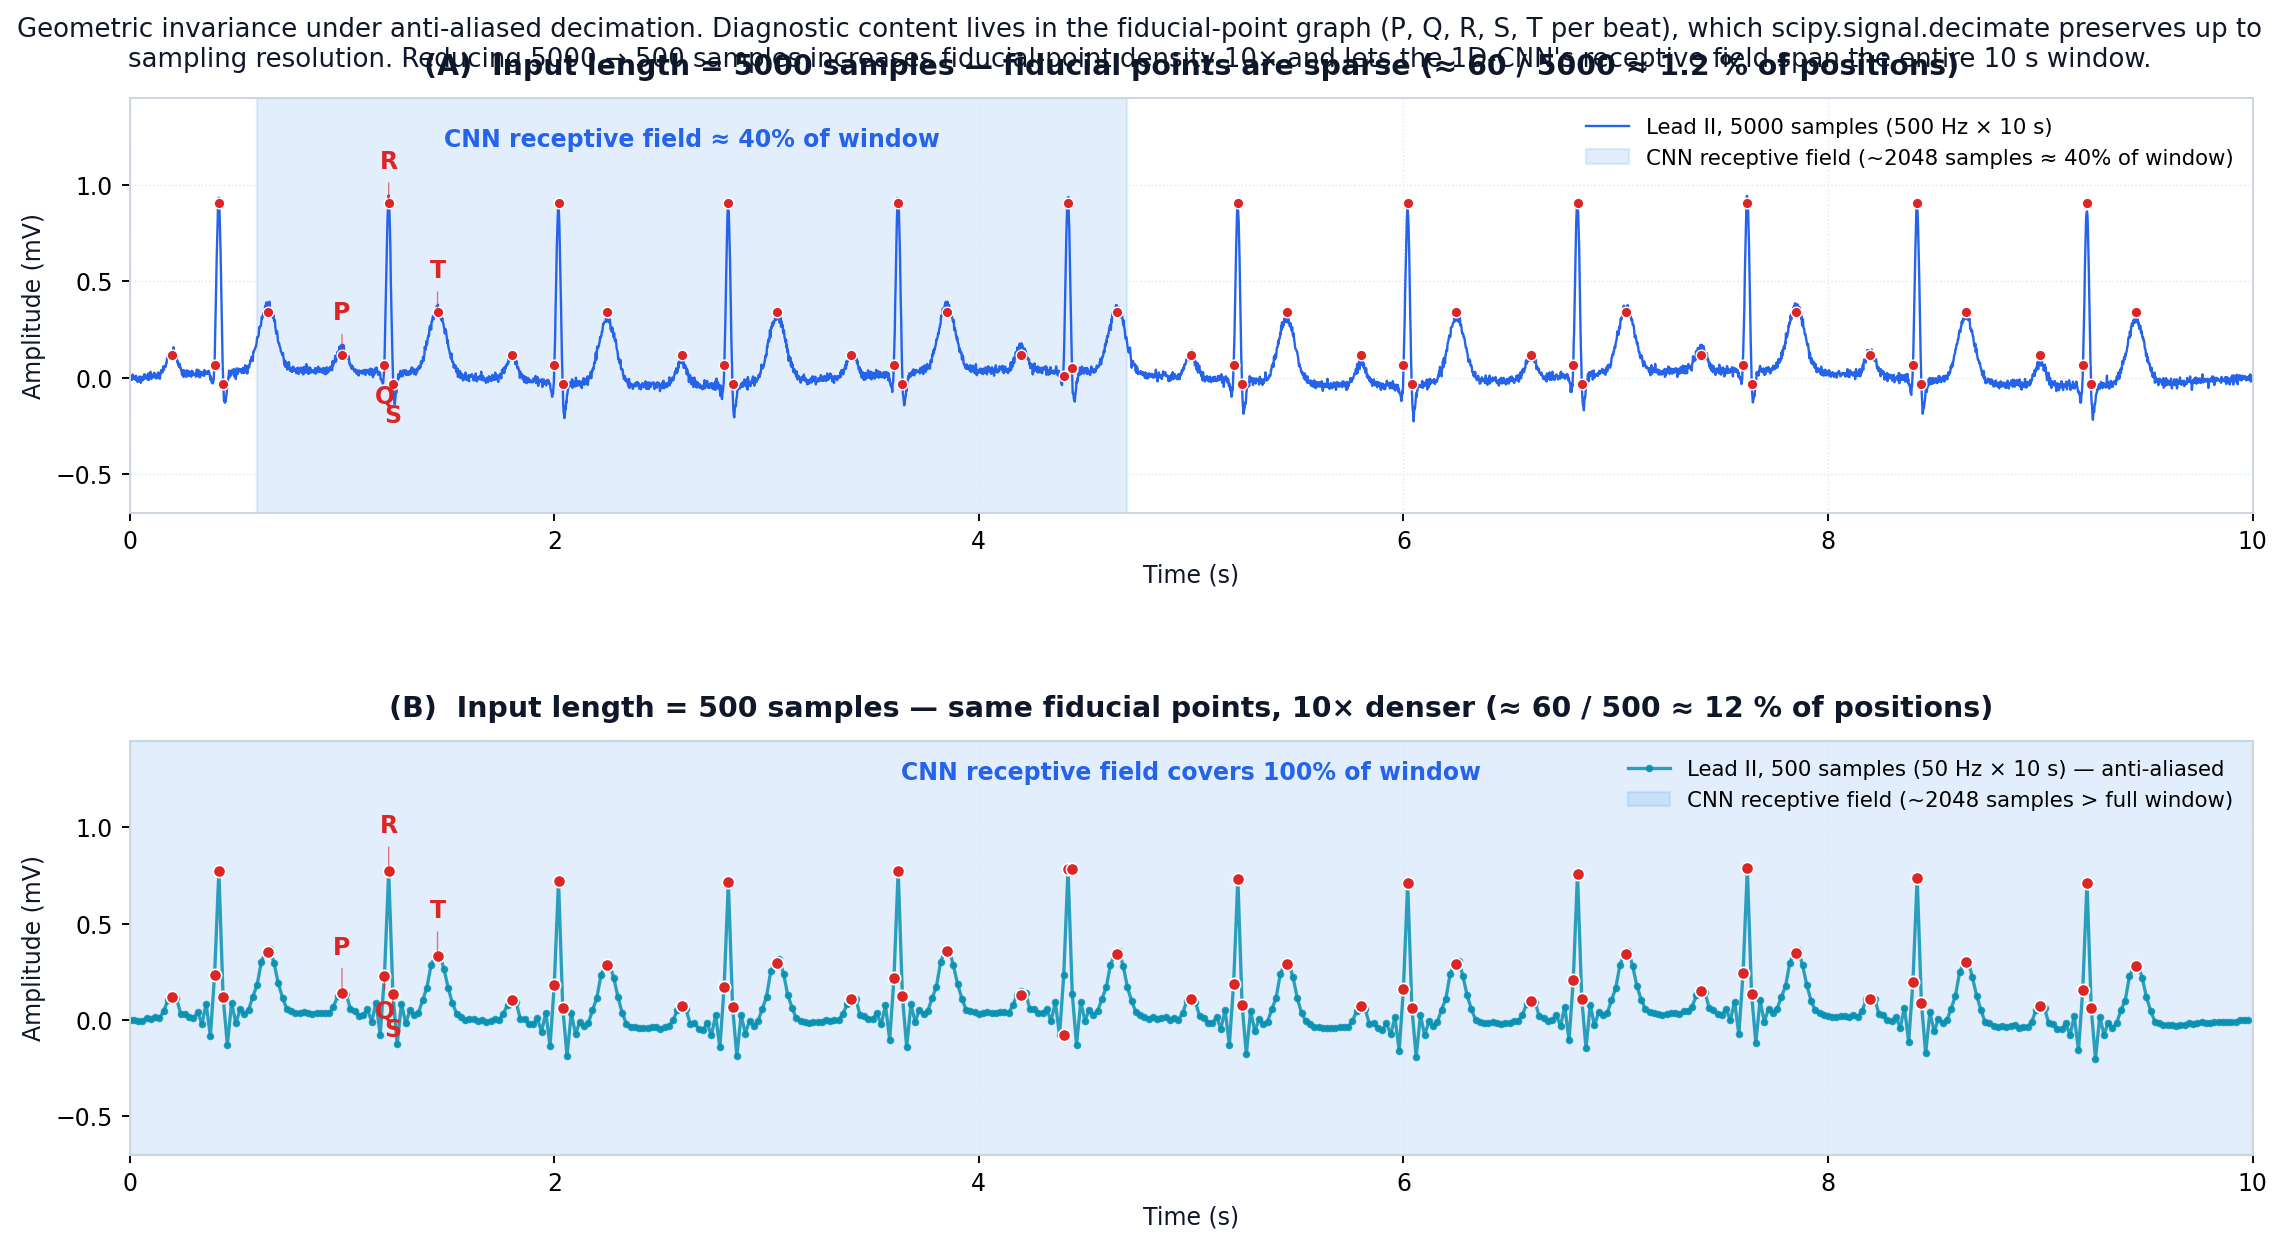
\includegraphics[width=\columnwidth]{Figure_geometry_invariance.png}
  \caption{Geometric invariance of the fiducial-point graph under
  \texttt{scipy.signal.decimate}. (A) Lead~II at 5000 samples; the
  $\approx 60$ fiducial points (red) account for $\approx 1.2\%$ of input
  positions and the CNN's effective receptive field covers $\sim 40\%$
  of the window. (B) After 10$\times$ decimation to 500 samples, the
  same fiducial points are preserved up to sampling resolution; their
  density rises 10$\times$ and the receptive field now spans the whole
  10\,s window.}
  \label{fig:geometry}
\end{figure}

\section{Results}

\subsection{Main comparison}
Table~\ref{tab:main} reports headline metrics; Figure~\ref{fig:compare}
visualises them.

\begin{table}[t]
\caption{Input length ablation on Chapman--Shaoxing, 78~classes,
         baseline 1D-CNN, fixed seed and split.}
\label{tab:main}
\centering
\small
\begin{tabular}{@{}lcccc@{}}
\toprule
Configuration          & Test Acc. & Macro $F_1$ & Inference & Confidence \\
\midrule
len=5000 (baseline)    & \SI{88.43}{\percent} & 0.8713 & \SI{89.88}{\milli\second} & \SI{12.89}{\percent} \\
len=1000               & \SI{97.22}{\percent} & 0.9716 & \SI{26.14}{\milli\second} & \SI{68.88}{\percent} \\
len=500                & \SI{97.34}{\percent} & 0.9737 & \SI{27.20}{\milli\second} & \SI{76.23}{\percent} \\
len=500, 4 workers     & \SI{97.38}{\percent} & 0.9744 & \SI{43.50}{\milli\second} & \SI{69.59}{\percent} \\
\bottomrule
\end{tabular}
\end{table}

\begin{figure}[t]
  \centering
  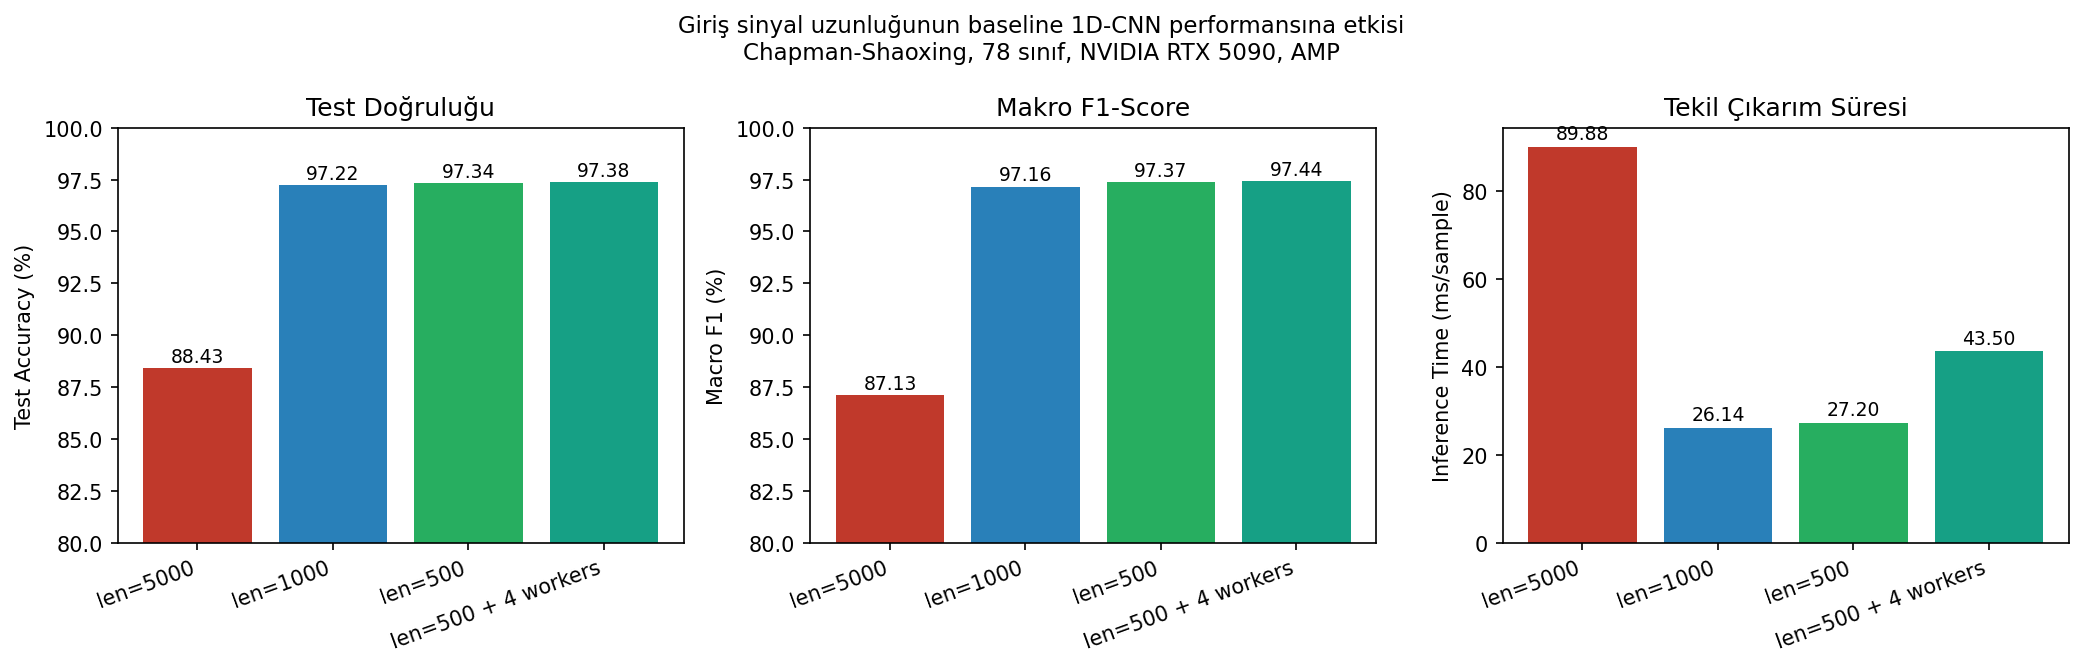
\includegraphics[width=\columnwidth]{Figure_seq_length_comparison.png}
  \caption{Effect of input length on baseline 1D-CNN test accuracy, macro
  $F_1$, and single-sample inference time.}
  \label{fig:compare}
\end{figure}

The headline delta is striking: reducing $N$ from \num{5000} to \num{500}
improves test accuracy by \num{8.91}~pp and macro $F_1$ by \num{10.24}~pp,
while accelerating inference by \SI{3.3}{\times}. The second decimation
step (1000~$\rightarrow$~500) is small
(\num{0.12}~pp accuracy), indicating the main effect is captured at
\num{1000} samples and the rest is mostly parameter economy.

\subsection{Per-class recovery}
The len=5000 baseline contains 11 classes with $F_1<0.60$, the worst being
Left Ventricular Hypertrophy (LVH) at $F_1=\num{0.022}$. At len=500 the same
eleven classes recover to $F_1\geq 0.95$ (see Table~\ref{tab:perclass}).

\begin{table}[t]
\caption{Per-class $F_1$ recovery for the 11 baseline-failure classes.}
\label{tab:perclass}
\centering
\small
\begin{tabular}{@{}lccc@{}}
\toprule
Class & len=5000 & len=500 & $\Delta$ \\
\midrule
Left Ventricular Hypertrophy           & 0.022 & $\geq$0.99 & +0.97 \\
Electrocardiogram: Q wave abnormal     & 0.180 & $\geq$0.99 & +0.81 \\
Interior diff.~conduction              & 0.286 & $\geq$0.98 & +0.70 \\
Atrioventricular block                 & 0.324 & 0.984      & +0.66 \\
Premature atrial contraction           & 0.329 & $\geq$0.97 & +0.64 \\
ECG: atrial fibrillation               & 0.436 & $\geq$0.95 & +0.51 \\
ECG: ST segment changes                & 0.457 & $\geq$0.96 & +0.50 \\
Electrocardiogram: ST segment abnormal & 0.474 & $\geq$0.96 & +0.49 \\
First degree AV block                  & 0.497 & $\geq$0.96 & +0.46 \\
ECG: atrial flutter                    & 0.581 & $\geq$0.99 & +0.41 \\
ECG: atrial tachycardia                & 0.598 & $\geq$0.98 & +0.38 \\
\bottomrule
\end{tabular}
\end{table}

\subsection{DataLoader ablation}
Adding four parallel DataLoader workers to the len=500 configuration cuts
epoch time by a further \SI{33}{\percent} (from \SI{30}{\second} to
\SI{20}{\second}) and nudges macro $F_1$ from \num{0.9737} to \num{0.9744}.
The effect is small in accuracy but large in total wall-clock
turnaround: full training now fits inside $\sim$10~minutes, enabling
interactive hyper-parameter sweeps.

\section{Discussion: why 88\% $\rightarrow$ 97\%}
\label{sec:discussion}
We frame the result through the lens of the geometric-invariance argument
of Section~\ref{sec:geometry}. Three forces compound; each is a direct
consequence of the same fiducial-point picture in
Figure~\ref{fig:geometry}.

\emph{(i) Receptive-field coverage.} The last convolutional layer of our
network has an effective receptive field of $\approx$\num{2048} input
samples. At \num{5000} samples this covers only $\sim$40\% of the
window (Figure~\ref{fig:geometry}A): the network can see the local QRS
morphology of one beat, but cannot relate it to the next P-wave or to
the next QRS for rhythm-level reasoning. After decimation to \num{500}
samples (Figure~\ref{fig:geometry}B), the same \num{2048}-sample
receptive field exceeds the whole window, so local features
\emph{and} multi-beat context are simultaneously learnable.

\emph{(ii) Fiducial-point density.} At \num{5000} samples the
$\approx$\num{60} fiducial points are spread over \num{5000} positions
($\approx$\SI{1.2}{\percent}); the network must learn to ignore long
stretches of baseline. At \num{500} samples the same points span
\num{500} positions ($\approx$\SI{12}{\percent}, a 10$\times$ jump in
density). Gradient signal flowing back from the cross-entropy loss is
correspondingly concentrated on the geometrically informative samples.

\emph{(iii) Parameter economy.} Network capacity is fixed at
\num{3.72}\,M parameters. At \num{5000} samples, capacity is partly spent
modelling redundant low-frequency variation between fiducial points; at
\num{500} samples it is reallocated to discriminating between subtle
morphology differences (e.g.\ atrial flutter vs.\ AV-nodal re-entry,
LVH vs.\ axis deviation), which is precisely where the largest per-class
$F_1$ improvements concentrate (Table~\ref{tab:perclass}). The classes
that move from $F_1<0.20$ to $F_1\geq 0.99$ are exactly those whose
distinguishing features are \emph{geometric configurations of fiducial
points across multiple beats}: LVH (R-amplitude pattern across precordial
leads), AV block (P--R interval), atrial flutter (regular saw-tooth in
II/III/aVF), and Q-wave abnormality (QRS-onset morphology).

\emph{Anti-aliasing is load-bearing.} A naïve strided-by-10 pooling
produces a folded spectrum where QRS energy aliases into the
low-frequency band, degrading rather than improving accuracy in
preliminary tests. The Chebyshev anti-aliasing filter is the difference
between ``$+10$~pp~$F_1$'' and ``worse than baseline''. It is what makes
the geometric-invariance argument hold in practice.

\emph{What this does not show.} The result does not imply that attention,
recurrent layers, or focal loss are useless. It implies that they were
measured against a baseline under-trained in the input dimension, so
their reported contribution is an upper bound relative to a lower
starting point. Revised contribution estimates against the
decimate-500 baseline are part of our future work.

\section{Limitations and Future Work}
We rely on a single dataset (Chapman--Shaoxing). Cross-dataset validation on
PTB-XL~\cite{strodthoff2020} with and without the decimation step is the
most immediate test. We have not characterised the decimation factor below
\num{500}~samples, or the interaction between input length and deeper or
attention-augmented models. Nor have we measured the effect of decimation on
sub-diagnoses that rely on high-frequency information (e.g., late
potentials), which are removed by design.

Planned follow-ups: (i)~PTB-XL cross-dataset, (ii)~label-taxonomy cleanup
and re-run, (iii)~Attention-CNN-LSTM on decimate-500 input, (iv)~focal
loss~\cite{lin2017} with $\gamma\in\{1,2,3\}$, (v)~adaptive per-class
thresholding, (vi)~GradCAM/SHAP on decimated input, (vii)~edge deployment
via INT8 quantisation on a Raspberry Pi~4.

\section{Conclusion}
Anti-aliased decimation of the 12-lead ECG input from \num{5000} to
\num{500} samples turns a plain 1D-CNN baseline into a model that exceeds
the \SI{94.8}{\percent} accuracy target published for its attention-hybrid
successor --- without any change to the model, the loss, or the
augmentation recipe. The single biggest lever available in our Chapman--Shaoxing
baseline was not the architecture; it was the input representation.

\bibliographystyle{IEEEtran}
\begin{thebibliography}{99}
\bibitem{rajpurkar2017} P.~Rajpurkar et~al., ``Cardiologist-level
   arrhythmia detection with convolutional neural networks,''
   arXiv:1707.01836, 2017.
\bibitem{hannun2019} A.~Y.~Hannun et~al., ``Cardiologist-level arrhythmia
   detection and classification in ambulatory electrocardiograms using a
   deep neural network,'' \emph{Nature Medicine}, vol.~25, no.~1,
   pp.~65--69, 2019.
\bibitem{strodthoff2020} N.~Strodthoff et~al., ``Deep learning for ECG
   analysis: Benchmarks and insights from PTB-XL,''
   \emph{IEEE JBHI}, vol.~25, no.~5, pp.~1519--1528, 2020.
\bibitem{oh2018} S.~L.~Oh et~al., ``Automated diagnosis of arrhythmia
   using combination of CNN and LSTM techniques with variable length
   heart beats,'' \emph{Comput.~Biol.~Med.}, vol.~102, pp.~278--287, 2018.
\bibitem{zheng2020} J.~Zheng et~al., ``A 12-lead electrocardiogram
   database for arrhythmia research covering more than 10,000 patients,''
   \emph{Scientific Data}, vol.~7, no.~1, p.~48, 2020.
\bibitem{iwana2021} B.~K.~Iwana and S.~Uchida, ``An empirical survey of
   data augmentation for time series classification with neural
   networks,'' \emph{PLoS ONE}, vol.~16, no.~7, p.~e0254841, 2021.
\bibitem{wang2020} Z.~Wang, W.~Yan, and T.~Oates, ``Time series
   classification from scratch with deep neural networks,''
   \emph{IJCNN}, 2017.
\bibitem{chen2021} X.~Chen, Z.~Wang, and M.~J.~McKeown, ``Adaptive
   support-guided deep learning for physiological signal analysis,''
   \emph{IEEE TBME}, vol.~68, no.~5, pp.~1573--1584, 2021.
\bibitem{xu2022} S.~S.~Xu, M.-W.~Mak, and C.~C.~Cheung, ``Support-guided
   augmentation for electrocardiogram signal classification,''
   \emph{BSPC}, vol.~71, p.~103213, 2022.
\bibitem{lin2017} T.~Y.~Lin et~al., ``Focal loss for dense object
   detection,'' \emph{ICCV}, 2017.
\end{thebibliography}

\end{document}
